\begin{question}
\noindent Shape $Q$ is shown on the grid below.

\begin{center}
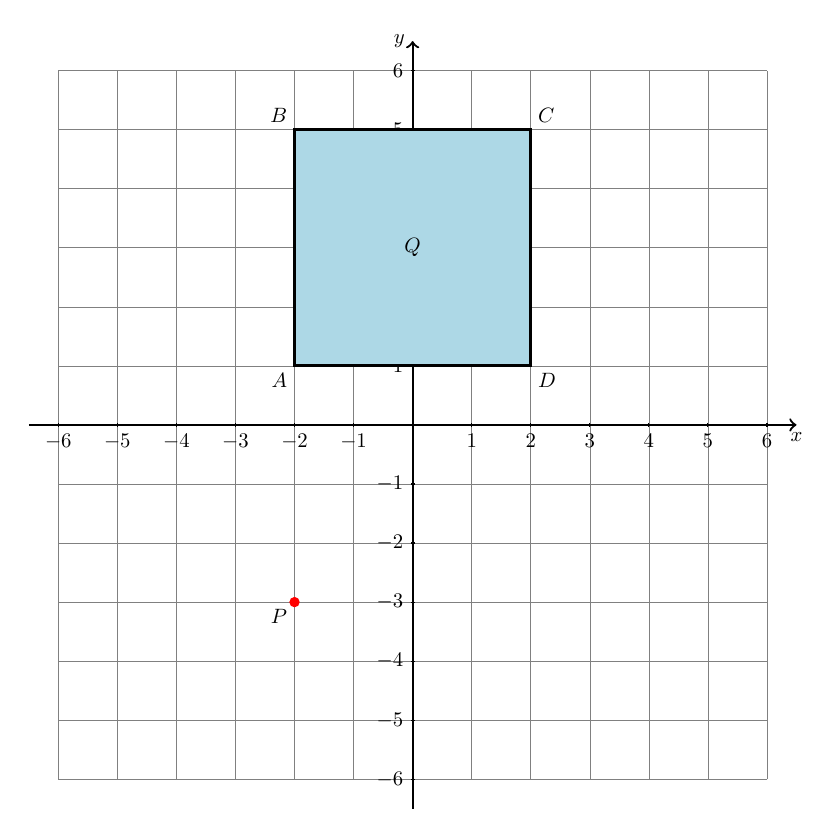
\begin{tikzpicture}[scale=0.75, transform shape]
    \definecolor{borderColour}{HTML}{000000}
    \definecolor{fillColourQ}{HTML}{ADD8E6}

    \def\axisLimit{6}

    % Draw grid
    \draw[step=1cm,gray,very thin] (-\axisLimit,-\axisLimit) grid (\axisLimit,\axisLimit);

    % Draw axes
    \draw[thick,->] (-\axisLimit-0.5,0) -- (\axisLimit+0.5,0) node[anchor=north] {$x$};
    \draw[thick,->] (0,-\axisLimit-0.5) -- (0,\axisLimit+0.5) node[anchor=east] {$y$};

    % Label x-axis and y-axis
    \foreach \x in {-\axisLimit,...,-1,1,2,...,\axisLimit}
        \draw (\x cm,1pt) -- (\x cm,-1pt) node[anchor=north] {$\x$};
    \foreach \y in {-\axisLimit,...,-1,1,2,...,\axisLimit}
        \draw (1pt,\y cm) -- (-1pt,\y cm) node[anchor=east] {$\y$};

    % Define vertices of Q
    \coordinate (A) at (-2,1);
    \coordinate (B) at (-2,5);
    \coordinate (C) at (2,5);
    \coordinate (D) at (2,1);

    % Draw Q
    \draw[fill=fillColourQ, draw=borderColour, line width=1pt] (A) -- (B) -- (C) -- (D) -- cycle;
    \node at (0,3) {$Q$};
    \node[below left] at (A) {$A$};
    \node[above left] at (B) {$B$};
    \node[above right] at (C) {$C$};
    \node[below right] at (D) {$D$};

    % Mark centre of enlargement
    \coordinate (P) at (-2,-3);
    \fill[red] (P) circle (2.5pt);
    \node[below left] at (P) {$P$};

\end{tikzpicture}
\end{center}

\noindent Rectangle $Q$ has vertices $A(-2,1)$, $B(-2,5)$, $C(2,5)$ and $D(2,1)$.

\noindent On the grid, enlarge rectangle $Q$ by scale factor $\dfrac{1}{2}$, centre $P(-2,-3)$.

\noindent Label the image $Q'$ and write down the coordinates of its vertices.

\vspace{5cm}

\begin{flushright}
    \answerplain{3}
\end{flushright}
\end{question}
